
\de{ĐỀ THI HỌC KỲ I NĂM HỌC 2022-2023}{THPT Trần Hưng Đạo}
\begin{center}
	\textbf{PHẦN 1 - TRẮC NGHIỆM}
\end{center}
\Opensolutionfile{ans}[ans/ans]

%Câu 1...........................
\begin{ex}%[Dự án đề kiểm tra HKI NH22-23- Nguyễn Võ Diễm Thy]%[THPT Trần Hưng Đạo]%[0T5Y2-1]
	Cho các điểm phân biệt $A$, $B$, $C$. Đẳng thức nào sau đây đúng?
	\choice
	{\True $\overrightarrow{AB}=\overrightarrow{AC}+\overrightarrow{CB}$}
	{$\overrightarrow{AB}=\overrightarrow{BC}-\overrightarrow{AC}$}
	{$\overrightarrow{AB}=\overrightarrow{CA}+\overrightarrow{BC}$}
	{$\overrightarrow{AB}=\overrightarrow{CB}-\overrightarrow{AC}$}
	\loigiai{
		Theo quy tắc ba điểm, ta có $\overrightarrow{AB}=\overrightarrow{AC}+\overrightarrow{CB}$.
	}
\end{ex}
\begin{ex}%[Dự án đề kiểm tra HKI NH22-23- Nguyễn Võ Diễm Thy]%[THPT Trần Hưng Đạo]%[0T3Y1-1]
	Đồ thị của hàm số $y=f(x)=\heva{&-2x+6& \text{ khi } x\le 1\\&4 &\text{ khi }x>1}$ đi qua điểm nào sau đây?
	\choice
	{\True $M\left(0;6\right)$}
	{$P\left(2;-3\right)$}
	{$N\left(1;-4\right)$}
	{$Q\left(0;4\right)$}
	\loigiai{
		Với $x=0$, ta có $f(0)=-2\cdot 0+6=6$ nên điểm $M(0;6)$ thuộc đồ thị hàm số $y=f(x)$.
	}
\end{ex}
\begin{ex}%[Dự án đề kiểm tra HKI NH22-23- Nguyễn Võ Diễm Thy]%[THPT Trần Hưng Đạo]%[0T4Y2-1]
	Cho tam giác $ABC$ có $AB=4$, $BC=8$, $\widehat{B}=60^\circ$. Tính độ dài cạnh $AC$.
	\choice
	{$4\sqrt{7}$}
	{$2\sqrt{3}$}
	{$2\sqrt{7}$}
	{\True $4\sqrt{3}$}
	\loigiai{
		Ta có $AC^2=AB^2+BC^2-2AB\cdot BC\cdot \cos B=48\Rightarrow AC=4\sqrt{3}$.
	}
\end{ex}
\begin{ex}%[Dự án đề kiểm tra HKI NH22-23- Nguyễn Võ Diễm Thy]%[THPT Trần Hưng Đạo]%[0T4Y2-1]
	Cho tam giác $ABC$ có $\widehat{A}=15^\circ$, $c=3$, $\widehat{B}=45^\circ$. Bán kính đường tròn ngoại tiếp của tam giác $ABC$ là
	\choice
	{$R=3\sqrt{3}$}
	{\True $R=\sqrt{3}$}
	{$R=2\sqrt{3}$}
	{$R=4\sqrt{3}$}
	\loigiai{
		Ta có $\widehat{C}=180^\circ-\widehat{A}-\widehat{B}=120^\circ$.\\
		Theo định lí sin, ta có $R=\dfrac{c}{2\sin C}=\dfrac{3}{2\sin 120^\circ}=\sqrt{3}$.
	}
\end{ex}
\begin{ex}%[Dự án đề kiểm tra HKI NH22-23- Nguyễn Võ Diễm Thy]%[THPT Trần Hưng Đạo]%[0T3Y1-4]
	Cho hàm số $y=f(x)$ có tập xác định $[-1;9]$ và đồ thị của nó như hình dưới đây.
	\begin{center}
		\begin{tikzpicture}[scale=0.6, font=\footnotesize, line join=round, line cap=round, >=stealth]
			\tikzset{label style/.style={font=\footnotesize}}
			%Nhập giới hạn đồ thị và hàm số cần vẽ
			\def \xmin{-2}
			\def \xmax{10}
			\def \ymin{-3}
			\def \ymax{7}
			\def \hamso{sin(\x r)}
			%\def \tiemcanxien{\x+1}
			%Tự động
			\draw[->] (\xmin,0)--(\xmax,0) node[below left] {$x$};
			\draw[->] (0,\ymin)--(0,\ymax) node[below left] {$y$};
			\draw[fill=black] (0,0) circle(1pt) node [below right] {$O$};
			%Vẽ các điểm trên 2 hệ trục
			\foreach \x in {-2,-1,1,2,3,4,6,7,8,9}
			\draw[fill=black] (\x,0) circle(1pt) node [below] {$\x$};
			\foreach \y in {-2,1,3,4,5,6}
			\draw[fill=black] (0,\y) circle(1pt) node [left] {$\y$};
			\draw[fill=black] (5,0) circle(1pt) node[above]{$5$};
			\draw[fill=black] (0,2) circle(1pt) node[right]{$2$};
			%Vẽ thêm mấy cái râu ria
			\draw[dashed,thin]
			(1,0)--(1,4)--(0,4)
			(5,0)--(5,-2)--(0,-2)
			(9,0)--(9,6)--(0,6)
			;
			\draw 
			(-1,0) ..controls +(82:0.1) and +(180:1.1)..
			(1,4) ..controls +(0:1.1) and +(120:0.4)..
			(4,0) ..controls +(-58:0.1) and +(180:0.1)..
			(5,-2)--(9,6)
			;
		\end{tikzpicture}
	\end{center}
	Khẳng định nào sau đây đúng?
	\choice
	{Hàm số đồng biến trên $(4;9)$}
	{Hàm số đồng biến trên $(-1;5)$}
	{\True Hàm số nghịch biến trên $(1;5)$}
	{Hàm số nghịch biến trên $(1;6)$}
	\loigiai{
		Từ đồ thị, ta thấy hàm số nghịch biến trên khoảng $(1;5)$ và đồng biến trên khoảng $(-1;1)$ và $(5;9)$.
	}
\end{ex}
\begin{ex}%[Dự án đề kiểm tra HKI NH22-23- Nguyễn Võ Diễm Thy]%[THPT Trần Hưng Đạo]%[0T3Y1-2]
	Tập xác định của hàm số $y=\dfrac{x-3}{x^2-4x+3}$ là
	\choice
	{$\mathscr{D}=\mathbb{R}\setminus\{3\}$}
	{$\mathscr{D}=\mathbb{R}\setminus\{1\}$}
	{$\mathscr{D}=\mathbb{R}\setminus\{-3;-1\}$}
	{\True $\mathscr{D}=\mathbb{R}\setminus\{3;1\}$}
	\loigiai{
		Hàm số xác định khi $x^2-4x+3\ne 0\Leftrightarrow \heva{& x\ne 1 \\ & x\ne 3.}$\\
		Vậy tập xác định $\mathscr{D}=\mathbb{R}\setminus\{3;1\}$.
	}
\end{ex}
\begin{ex}%[Dự án đề kiểm tra HKI NH22-23- Nguyễn Võ Diễm Thy]%[THPT Trần Hưng Đạo]%[0T1Y1-3]
	Mệnh đề phủ định của mệnh đề $P\colon \text{\lq\lq}\forall x\in \mathbb{R}, x^2\ge 0\text{\rq\rq}$ là
	\choice
	{\True $\overline{P}\colon \text{\lq\lq}\exists x\in \mathbb{R}, x^2<0\text{\rq\rq}$}
	{$\overline{P}\colon \text{\lq\lq}\forall x\in \mathbb{R}, x^2<0\text{\rq\rq}$}
	{$\overline{P}\colon \text{\lq\lq}\forall x\in \mathbb{R}, x^2\le 0\text{\rq\rq}$}
	{$\overline{P}\colon \text{\lq\lq}\exists x\in \mathbb{R}, x^2\ne 0\text{\rq\rq}$}
	\loigiai{
		Mệnh đề phủ định của mệnh đề $P\colon \text{\lq\lq}\forall x\in \mathbb{R}, x^2\ge 0\text{\rq\rq}$ là $\overline{P}\colon \text{\lq\lq}\exists x\in \mathbb{R}, x^2<0\text{\rq\rq}$.
	}
\end{ex}
\begin{ex}%[Dự án đề kiểm tra HKI NH22-23- Nguyễn Võ Diễm Thy]%[THPT Trần Hưng Đạo]%[0T2Y1-1]
	Bất phương trình nào sau đây là bất phương trình bậc nhất hai ẩn?
	\choice
	{$x^2+4y^2\le 6$}
	{$xy+x+y>0$}
	{\True $2x-3y\ge -2$}
	{$x+y^2\ge 2$}
	\loigiai{
		Bất phương trình $2x-3y\ge -2$ là bất phương trình bậc nhất hai ẩn.
	}
\end{ex}
\begin{ex}%[Dự án đề kiểm tra HKI NH22-23- Nguyễn Võ Diễm Thy]%[THPT Trần Hưng Đạo]%[0T1Y2-3]
	Cho tập hợp $A=\{x\in \mathbb{R}|x\le 3\}$. Hãy viết tập hợp $A$ dưới dạng khoảng, đoạn, nửa khoảng
	\choice
	{$A=(-\infty;3)$}
	{\True $A=\left(-\infty;3\right]$}
	{$A=\left(3;+\infty\right)$}
	{$A=\left[3;+\infty\right)$}
	\loigiai{
		Vì $x\le 3$ nên $x\in \left(-\infty;3\right]$. Do đó $A=\left(-\infty;3\right]$.
	}
\end{ex}
\begin{ex}%[Dự án đề kiểm tra HKI NH22-23- Nguyễn Võ Diễm Thy]%[THPT Trần Hưng Đạo]%[0T1Y3-4]
	Cho hai tập hợp $A=(-6;0)$ và $B=(3;+\infty)$. Khẳng định nào sau đây đúng?
	\choice
	{$A\cup B=(0;+\infty)$}
	{$A\cap B=\left(-3;0\right]$}
	{$A\cap B=(-6;-3)$}
	{\True $A\cup B=(-6;+\infty)$}
	\loigiai{
		Biểu diễn hai tập hợp $A$ và $B$ lên trục số
		\begin{center}
			\begin{tikzpicture}[scale=1, font=\footnotesize, line join=round, line cap=round,>=stealth]%<DTools>
				\def\xmin{-10};\def\xmax{5};
				%(-6;0)
				\draw[->] (\xmin,0)--(\xmax,0);
				\node (a0) at (-6,{0}){(};
				\node (b0) at (0,0){)};
				\draw (a0.-90)node[below]{$-6$} (b0.-90)node[below]{$0$};
				\draw[draw=none, pattern=north west lines] ($(a0)+(90:0.1)$)--(\xmin,0.1)--(\xmin,-0.1)--($(a0)+(-90:0.1)$) ($(b0)+(90:0.1)$)--(\xmax,0.1)--(\xmax,-0.1)--($(b0)+(-90:0.1)$);
				%(-3;+oo)
				\draw[->] (\xmin,-1)--(\xmax,-1);
				\node (a1) at (-3,{-1}){(};
				\draw (a1.-90)node[below]{$-3$};
				\draw[draw=none, pattern=north west lines] ($(a1)+(90:0.1)$)--(\xmin,{0.1-1})--(\xmin,{-0.1-1})--($(a1)+(-90:0.1)$);
			\end{tikzpicture}
		\end{center}
		Từ đó, ta thấy $A\cup B=(-6;+\infty)$.
	}
\end{ex}

%Câu 11...........................
	\begin{ex}%[0T2Y2-3]%[Dự án đề kiểm tra HKII NH22-23- Mui Doan]%[THPT Trần Hưng Đạo]
		Cho hệ bất phương trình bậc nhất hai ẩn $\heva{&x-y\le -3\\&2y\ge -4}$. Điểm nào sau đây thuộc miền nghiệm của hệ bất phương trình đã cho?
		\choice
		{\True $P(-3;1)$}
		{$N(-2;1)$}
		{$O(0;0)$}
		{$M(3;-1)$}
		\loigiai{
		\begin{itemize}
			\item Thế tọa độ của $P(-3;1)$ vào hệ ta được $\heva{&-3-1\le -3\\&2\cdot 1\ge -4}$ đúng.\\ Suy ra điểm $P(-3;1)$ thuộc miền nghiệm của hệ bất phương trình đã cho.
			\item Thế tọa độ của $N(-2;-1)$ vào hệ ta được $\heva{&-2-(-1)\le -3\\&2\cdot 1\ge -4}$ sai.\\ Suy ra điểm $N(-2;1)$ không thuộc miền nghiệm của hệ bất phương trình đã cho.
			\item Thế tọa độ của $O(0;0)$ vào hệ ta được $\heva{&0-0\le -3\\&2\cdot 0\ge -4}$ sai.\\ Suy ra điểm $O(0;0)$ không thuộc miền nghiệm của hệ bất phương trình đã cho.
			\item Thế tọa độ của $M(3;-1)$ vào hệ ta được $\heva{&3-(-1)\le -3\\&2\cdot (-1)\ge -4}$ sai.\\ Suy ra điểm $M(3;-1)$ không thuộc miền nghiệm của hệ bất phương trình đã cho.
		\end{itemize}	
		}
	\end{ex}
	%Câu 12...........................
	\begin{ex}%[0T2B1-2]%[Dự án đề kiểm tra HKII NH22-23- Mui Doan]%[THPT Trần Hưng Đạo]
		\immini{
			Miền không tô đậm ở hình vẽ dưới đây là biểu diễn miền nghiệm của bất phương trình nào?
			\choice
			{$2x-y+4\le 0$}
			{\True $2x-y+4\ge 0$}
			{$2x+y+4\ge 0$}
			{$2x+y+4\le 0$}
		}{
			\begin{tikzpicture}[scale=.6, font=\footnotesize, line join=round, line cap=round, >=stealth]
				\draw[->] (-3,0)--(2,0) node [below]{$x$};
				\draw[->] (0,-1)--(0,5) node [left]{$y$};
				\draw[fill=black] (0,0) circle(1pt) node[below right]{$O$};
				\begin{scope}
					\clip (-3+0.01,-1+0.01) rectangle (2-0.01,5-0.01);
					\draw[samples=350,domain=-3+0.01:5-0.01,smooth,variable=\x] plot (\x,{2*(\x)+4});
					\fill[draw, pattern=north west lines] (-3,-2)--(2,8)--(-3,8)--cycle;
				\end{scope}
				\draw[fill=black] (-2,0) circle(1pt) node[below right]{$-2$};
				\draw[fill=black] (0,4) circle(1pt) node[below right]{$4$};
			\end{tikzpicture}
		}
		\loigiai{
		Đường thẳng đi qua hai điểm $(-2;0)$  và $(0;4)$ là $2x-y+4=0$.\\
		Ta có $2\cdot 0-0+4>0$ nên miền chứa điểm $O$ là miền nghiệm của bất phương trình $2x-y+4\ge 0$.
		}
	\end{ex}
	%Câu 13...........................
	\begin{ex}%[0T2Y1-2]%[Dự án đề kiểm tra HKII NH22-23- Mui Doan]%[THPT Trần Hưng Đạo]
		Trong các cặp số sau đây, cặp số $(x;y)$ nào sau đây thuộc miền nghiệm của bất phương trình $2x-3y+5>0$?
		\choice
		{$(-3;2)$}
		{$(-5;0)$}
		{\True $(0;0)$}
		{$(-2;1)$}
		\loigiai{
		\begin{itemize}
			\item Thế cặp số $(-3;2)$ vào bất phương trình ta được $2\cdot (-3)-3\cdot 2+5>0$ sai.\\
			Suy ra cặp số $(-3;2)$ không thuộc miền nghiệm của bất phương trình $2x-3y+5>0$.
			\item Thế cặp số $(-5;0)$ vào bất phương trình ta được $2\cdot (-5)-3\cdot 0+5>0$ sai.\\
			Suy ra cặp số $(-5;0)$ không thuộc miền nghiệm của bất phương trình $2x-3y+5>0$.
			\item Thế cặp số $(0;0)$ vào bất phương trình ta được $2\cdot 0-3\cdot 0+5>0$ đúng.\\
			Suy ra cặp số $(0;0)$  thuộc miền nghiệm của bất phương trình $2x-3y+5>0$.
			\item Thế cặp số $(-2;1)$ vào bất phương trình ta được $2\cdot (-1)-3\cdot 1+5>0$ sai.\\
			Suy ra cặp số $(-2;1)$ không thuộc miền nghiệm của bất phương trình $2x-3y+5>0$.
		\end{itemize}	
		}
	\end{ex}
	%Câu 14...........................
	\begin{ex}%[0T3Y2-3]%[Dự án đề kiểm tra HKII NH22-23- Mui Doan]%[THPT Trần Hưng Đạo]
		Phương trình trục đối xứng của parabol $y=2x^2-6x+1$ là
		\choice
		{$x=-\dfrac{3}{2}$}
		{$x=3$}
		{$x=\dfrac{1}{2}$}
		{\True $x=\dfrac{3}{2}$}
		\loigiai{
		Phương trình trục đối xứng của parabol $y=2x^2-6x+1$ là $x=-\dfrac{b}{2a}= \dfrac{3}{2}$.	
		}
	\end{ex}
	%Câu 15...........................
	\begin{ex}%[0T6Y1-2]%[Dự án đề kiểm tra HKII NH22-23- Mui Doan]%[THPT Trần Hưng Đạo]
		Cho biết $\sqrt[3]{3}=1{,}44224957...$. Số gần đúng của $\sqrt[3]{3}$ với độ chính xác $d=0{,}0001$ là
		\choice
		{$1{,}4421$}
		{\True $1{,}4422$}
		{$1{,}442$}
		{$1{,}44$}
		\loigiai{
		Vì độ chính xác là $d=0{,}0001$ với chữ số bên phải đầu tiên khác $0$	ở phần chục nghìn nên số gần đúng là $1{,}4422$.
		}
	\end{ex}
	%Câu 16...........................
	\begin{ex}%[0T2Y2-1]%[Dự án đề kiểm tra HKII NH22-23- Mui Doan]%[THPT Trần Hưng Đạo]
		Hệ bất phương trình nào sau đây \textbf{không} phải là hệ bất phương trình bậc nhất hai ẩn?
		\choice
		{$\heva{&x>3\\&y\le -4}$}
		{$\heva{&x-2y\le 3\\&x+2y\ge 4}$}
		{\True $\heva{&3x+y<4\\&x^2+y>3}$}
		{$\heva{&y>0\\&x+y\le 0}$}
		\loigiai{
		Hệ bất phương trình \textbf{không} phải là hệ bất phương trình bậc nhất hai ẩn là 	$\heva{&3x+y<4\\&x^2+y>3}$.
		}
	\end{ex}
	%Câu 17...........................
	\begin{ex}%[0T1Y1-1]%[Dự án đề kiểm tra HKII NH22-23- Mui Doan]%[THPT Trần Hưng Đạo]
		Câu nào sau đây \textbf{không phải} là mệnh đề?
		\choice
		{$2+1>10$}
		{\True Bạn bao nhiêu tuổi rồi?}
		{$\sqrt{2}$ là một số vô tỉ}
		{$5$ là một số lẻ}
		\loigiai{
		\lq\lq Bạn bao nhiêu tuổi rồi?\rq\rq\, là câu hỏi nên \textbf{không phải} là mệnh đề.
		}
	\end{ex}
	%Câu 18...........................
	\begin{ex}%[0T4Y2-1]%[Dự án đề kiểm tra HKII NH22-23- Mui Doan]%[THPT Trần Hưng Đạo]
		Tam giác $ABC$ có $BC=a$, $AC=b$, $AB=c$ và bán kính đường tròn ngoại tiếp $R$. Đẳng thức nào sau đây đúng?
		\choice
		{$S=\dfrac{a+b+c}{4R}$}
		{$S=\dfrac{abc}{2R}$}
		{\True $S=\dfrac{abc}{4R}$}
		{$S=\dfrac{a+b+c}{2R}$}
		\loigiai{
		Đẳng thức đúng là 	$S=\dfrac{abc}{4R}$.
		}
	\end{ex}
	%Câu 19...........................
	\begin{ex}%[0T6B1-2]%[Dự án đề kiểm tra HKII NH22-23- Mui Doan]%[THPT Trần Hưng Đạo]
		Cho số gần đúng $a=2048$ với độ chính xác $d=50$. Số quy tròn của $a$ bằng bao nhiêu?
		\choice
		{\True $2000$}
		{$2040$}
		{$2050$}
		{$2100$}
		\loigiai{
		Vì độ chính xác  là độ chính xác $d=50$ nên ta làm tròn số $a$ ở hàng trăm.\\
		Số quy tròn của $a$ là $2000$.
		}
	\end{ex}
	%Câu 20...........................
	\begin{ex}%[0T5B3-3]%[Dự án đề kiểm tra HKII NH22-23- Mui Doan]%[THPT Trần Hưng Đạo]
		Trên đường thẳng $MN$ lấy điểm $P$ sao cho $\overrightarrow{MN}=-3\overrightarrow{MP}$. Điểm $P$ được xác định đúng trong hình vẽ nào sau đây?
		\begin{center}
			\begin{tikzpicture}[scale=1, font=\footnotesize, line join=round, line cap=round, >=stealth]
				\foreach \x in {-6,-5,-4,-3,-2,-1,2,3,4,5}
				\draw[fill=black] (\x,3) circle(1.5pt);
				\foreach \y in {-6,-5,-4,-3,-2,1,2,3,4,5}
				\draw[fill=black] (\y,1) circle(1.5pt);
				\path
				(-6,3) node[below]{$M$}
				(-3,3) node[below]{$P$}
				(-1,3) node[below]{$N$}
				(2,3) node[below]{$N$}
				(3,3) node[below]{$M$}
				(5,3) node[below]{$P$}
				(-6,1) node[below]{$N$}
				(-3,1) node[below]{$M$}
				(-2,1) node[below]{$P$}
				(1,1) node[below]{$M$}
				(4,1) node[below]{$P$}
				(5,1) node[below]{$N$}
				(-4,2) node{\text{Hình 1}}
				(3,2) node{\text{Hình 2}}
				(-4,0) node{\text{Hình 3}}
				(3,0) node{\text{Hình 4}}
				;
				\draw
				(-6,3)--(-1,3)
				(2,3)--(5,3)
				(-6,1)--(-2,1)
				(1,1)--(5,1)
				;
			\end{tikzpicture}
		\end{center}
		\choice
		{Hình $1$}
		{Hình $4$}
		{Hình $2$}
		{\True Hình $3$}
		\loigiai{
		Vì 	$\overrightarrow{MN}=-3\overrightarrow{MP}$ nên $\overrightarrow{MN}$ và $\overrightarrow{MP}$ ngược hướng và $\left\vert\overrightarrow{MN}\right\vert=3\left\vert\overrightarrow{MP}\right\vert$.
		Vậy Hình $3$ thỏa đề bài.
		}
	\end{ex}


\Closesolutionfile{ans}
%\begin{center}
%	\textbf{ĐÁP ÁN}
%	\inputansbox{10}{ans/ans}	
%\end{center}


\begin{center}
	\textbf{PHẦN 2 - TỰ LUẬN}
\end{center}

\begin{bt}%[0T3B2-2]
	Xác định hàm số $y=ax^2+bx+c$ ($a\ne 0$) biết đồ thị của hàm số là một parabol có đỉnh $I(1;1)$ và đi qua điểm $A(2;3)$.
\dapso{$y=2x^2-4x+3$}
\loigiai{
Theo giả thiết bài toán có đỉnh $ I(1;1) $ nên $ \heva{&\dfrac{-b}{2a}= 1\\&a+b+c=1.}$\\
Mà parabol đi qua điểm $ A(2;3) $ nên $ 4a+2b+c=3 $.\\
Do đó ta có hệ phương trình
$\heva{&2a+b=0\\&a+b+c=1\\&4a+2b+c=3}\Leftrightarrow \heva{&a=2\\&b=-4\\&c=3.} $\\
Vậy hàm số cần tìm là $ y=2x^2-4x+3 $.}
\end{bt}
\begin{bt}%[0T3K2-5]
\immini{Một cổng chào của sân vận động tỉnh A có hình dạng là một parabol hướng bề lõm xuống dưới. Giả sử ta gắn hệ tọa độ $Oxy$ sao cho một chân cổng đi qua gốc tọa độ $O$ như hình vẽ ($x, y$ tính bằng mét), chân kia của cổng ở vị trí có tọa độ $(4;0)$. Biết một điểm $M$ trên cổng có tọa độ $(3;12)$. Tính chiều cao của cổng ở vị trí cao nhất.
}{
	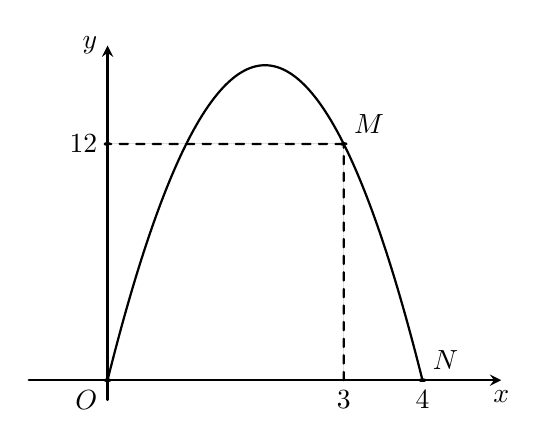
\begin{tikzpicture}[yscale=0.25, line join=round, line cap=round,>=stealth,thick]
		\draw[->] (-1,0) --(5,0) node[below]{$ x $};
		\draw[->](0,-1)--(0,17) node[left]{$ y $};
		\draw[fill=black] (0,0) circle (1pt) node [below left] {$O$};
		\begin{scope}
			\clip (-1,-1) rectangle (5,17);
			\draw[samples=200,domain=0:4,smooth,variable=\x] plot (\x,{-4*(\x)^2+16*(\x)+0});
		\end{scope}
	\draw[fill=black,dashed] (3,0) node[below] {$ 3 $} --(3,12) circle (1pt) node[above right]{$ M $}--(0,12) circle (1pt) node[left]{$ 12 $};
  \draw[fill=black] (4,0) circle (1pt) node[above right]{$ N $};
  \draw (4,0) node[below]{$ 4 $};
	\end{tikzpicture}
}

	\dapso{$16$m}
	
	\loigiai{
	 	Gọi phương trình parabol mô phỏng cho cổng có phương trình $ y=ax^2+bx+c $, $ a\ne0 $.\\
	 	Parabol  đi qua các điểm $ O(0;0) $, $ M(3;12) $, $ N(4,0) $ nên ta có hệ phương trình $$ \heva{& c=0\\&9a+3b+c=12\\&16a+4b+c=0}\Leftrightarrow \heva{&a=-4 \\&b=16\\&c=0.} $$
	 	Phương trình của parabol là $ y=-4x^2+16x $.\\
	 	Chiều cao của cổng ở vị trí cao nhất bằng tung tung độ đỉnh parabol $ y=-\dfrac{\Delta}{4a} =16$.
	}
\end{bt}
\begin{bt}%[0T2K2-2]
	Lớp 10A tham gia cuộc thi thiết kế thiệp mừng ngày Nhà giáo Việt Nam 20-11 do Đoàn thanh niên phát động và các tấm thiệp sẽ được nhà trường mua lại tặng các thầy cô giáo. Cần $1$ giờ để hoàn thành một tấm thiệp nhỏ có giá $15$ nghìn đồng và $3$ giờ để hoàn thành tấm thiệp loại lớn có giá $40$ nghìn đồng. Mỗi lớp chỉ có $6$ giờ để thiết kế và chỉ được dự thi không quá $4$ thiệp. Hãy cho biết lớp 10A cần làm bao nhiêu tấm thiệp mỗi loại để được tiền nhiều nhất?
	\dapso{$3$ thiệp loại nhỏ, $1$ thiệp loại lớn}
	\loigiai{
	\immini{	Gọi số thiệp loại nhỏ và thiệp loại lớn mà lớp 10A làm lần lượt là $ x $, $ y $ (với $ x,y\ge 0 $).\\
		Thời gian cần làm $ x $ thiệp nhỏ là $ x $ giờ.\\
		Thời gian cần làm $ y $ thiệp lớn là $ 3y $ giờ.\\
		Theo bài ra mỗi lớp chỉ có $ 6 $ giờ để làm thiệp nên $ x+3y\le 6 $.\\
		Mỗi lớp dự thi không quá $ 4 $ thiệp nên $ x+y\le 4 $.\\
		Tổng số tiền thu về là $ T(x;y)=15\cdot x +40\cdot y$ nghìn đồng.\\ 
		Như vậy yêu cầu bài toán đưa về việc tìm $ (x;y) $ thỏa mãn hệ $ \heva{&x\ge 0\\&y\ge 0\\&x+3y\le6\\&x+y\le 4} $ sao cho $ T(x;y) $ đạt giá trị lớn nhất.
		Miền nghiệm của hệ bất phương trình là tứ giác $ OABC $ với $ O(0;0) $, $ A(0,2) $, $ B(3,1) $, $ C(4,0) $.\\
		Ta có $ T(0,0)=0 $, $ T(0,2)=30 $, $ T(3,1) =85$ và $ T(4,0)=60 $.\\
		Do đó lớp 10A cần làm $ 3 $ thiệp loại nhỏ và $ 1 $ thiệp loại lớn
		 thì sẽ thu được số tiền nhiều nhất.}{
	 
			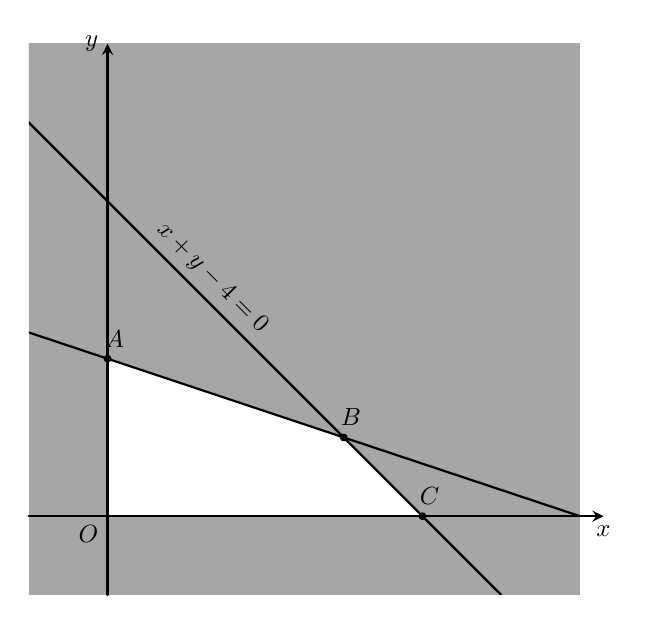
\begin{tikzpicture}[line join=round, line cap=round,>=stealth,thick]
				\tikzset{every node/.style={scale=0.9}}
				\begin{scope}
					\clip (-1,-1) rectangle (6,6);
					\fill[black!35] (0,-1)--(-1,-1)--(-1,6)--(0,6)--cycle;
					\fill[black!35] (-1,0)--(-1,-1)--(6,-1)--(6,0)--cycle;
					\fill[black!35] (-13,6.33)--(10,6.33)--(10,-1.33)--cycle;
					\fill[black!35] (-3,7)--(7,7)--(7,-3)--cycle;
					\draw (-12,6)--(9,-1) node [pos=0.45, above, sloped] {$x+3y-6=0$};
					\draw (-2,6)--(5,-1) node [pos=0.45, above, sloped] {$x+y-4=0$};
				\end{scope}
				\draw[->] (-1,0)--(6.3,0) node[below]{$x$};
				\draw[->] (0,-1)--(0,6) node[left]{$y$};
				\draw (0,0) node[below left]{$O$};
		\draw[fill=black] (0,2) circle (1pt) node[shift={(70:0.3)}]{$ A $};
		\draw[fill=black] (3,1) circle (1pt) node[shift={(70:0.3)}]{$ B $};
		\draw[fill=black] (4,0) circle (1pt) node[shift={(70:0.3)}]{$ C $};
		\end{tikzpicture}
	}
	}
\end{bt}

\begin{bt}%[0H5Y2-2]%[0H5Y2-5]%[Dự án đề kiểm tra HKI NH22-23 - Nguyễn Ngọc Dũng]%[THPT Trần Hưng Đạo]
\begin{enumerate}
\item Cho các điểm $A$, $B$, $C$, $D$, $E$. Chứng minh $\overrightarrow{AD}+\overrightarrow{BC}-\overrightarrow{EC}-\overrightarrow{BD}=\overrightarrow{AE}$.
\item Cho $\triangle ABC$ vuông tại $A$ có $AB=3$, $AC=4$. Gọi $H$ là trung điểm cạnh $BC$. Tính độ dài véc-tơ $\overrightarrow{HB}-\overrightarrow{HC}$.
\end{enumerate}
\dapso{b) $5$}
\loigiai{
\begin{enumerate}
\item Ta có
\allowdisplaybreaks 
\begin{eqnarray*}
\text{VT} &=& \overrightarrow{AD}+\overrightarrow{BC}-\overrightarrow{EC}-\overrightarrow{BD} \\
&=& \overrightarrow{AD}+\overrightarrow{BC}+\overrightarrow{CE}+\overrightarrow{DB}  \\
&=& \overrightarrow{AD}+\overrightarrow{DB}+\overrightarrow{BC}+\overrightarrow{CE} \\
&=&  \overrightarrow{AE} \text{ (đpcm)}.
\end{eqnarray*}
\item 
\immini{
Ta có $\left| \overrightarrow{HB}-\overrightarrow{HC} \right| = \left| \overrightarrow{CB} \right| =BC$.\\
Vì $\triangle ABC$ vuông tại $A$ nên 
$$BC=\sqrt{AB^2+AC^2} = \sqrt{3^2+4^2} = 5.$$
Vậy $\left| \overrightarrow{HB}-\overrightarrow{HC} \right| =5$.
}{
\begin{tikzpicture}[line cap=round, line join =round, >=stealth]
%\draw[cyan,dashed] (-5,-5) grid (5,5);
\coordinate[label={below left}:$B$] (B) at (-3,-2);
\coordinate[label={below right}:$C$] (C) at ($(B)+(5,0)$);
\coordinate[label={below}:{$H$}] (H) at ($(B)!0.5!(C)$);
\coordinate[label={above}:{$A$}] (A) at ($(H)!1!120:(C)$);
\draw (A)--(B)--(C)--cycle;

\draw
pic[draw, angle radius=2mm]{right angle=B--A--C}
;
\foreach \x in {A,B,C,H}
\draw[fill=black] (\x) circle (1pt);
\end{tikzpicture}
}
\end{enumerate}
}
\end{bt}

\begin{bt}%[0H5B4-1]%[Dự án đề kiểm tra HKI NH22-23 - Nguyễn Ngọc Dũng]%[THPT Trần Hưng Đạo]
\begin{enumerate}
\item Cho $\triangle ABC$ có $AB=2$, $BC=4$, $\widehat{ABC}=60^\circ$. Tính tích vô hướng $\overrightarrow{BA}\cdot \overrightarrow{BC}$.
\item Cho hình vuông $ABCD$ có tâm $O$ có độ dài cạnh bằng $a$. Tính tích vô hướng $\overrightarrow{AB}\cdot \overrightarrow{OC}$.
\end{enumerate}
\dapso{a) $4$;   b) $\dfrac{a^2}{2}$}
\loigiai{
\begin{enumerate}
\item Ta có $\overrightarrow{BA}\cdot \overrightarrow{BC} = BA\cdot BC \cdot \cos \widehat{ABC} = 2\cdot 4 \cdot \cos 60^\circ = 4$.
\item Ta có $AC=\sqrt{AB^2+AC^2} = a\sqrt{2}$ và $AO=\dfrac{AC}{2} = \dfrac{a\sqrt{2}}{2}$. Khi đó
\immini{
\allowdisplaybreaks 
\begin{eqnarray*}
\overrightarrow{AB}\cdot \overrightarrow{OC} &=& \overrightarrow{AB}\cdot \overrightarrow{AO} \\
&=& AB\cdot AO \cdot \cos \widehat{BAO} \\
&=& a\cdot \dfrac{a\sqrt{2}}{2} \cdot \cos 45^\circ	 \\
&=& \dfrac{a^2}{2}.
\end{eqnarray*}
}{
\begin{tikzpicture}[line cap=round, line join =round, >=stealth]
\def\r{3} \def\d{3}
\coordinate[label={below left}:$B$] (B) at (-3,-2);
\coordinate[label={above left}:$A$] (A) at ($(B)+(0,\r)$);
\coordinate[label={below right}:$C$] (C) at ($(B)+(\d,0)$);
\coordinate[label={above  right}:$D$] (D) at ($(A)+(\d,0)$);
\coordinate[label={above}:{$O$}] (O) at ($(A)!0.5!(C)$);
\draw (A)--(B)--(C)--(D)--(A)--(C) (B)--(D);
\draw
pic[draw, angle radius=2mm]{right angle=A--B--C}
pic[draw, angle radius=2mm]{right angle=A--D--C}
pic[draw, angle radius=2mm]{right angle=B--A--D}
pic[draw, angle radius=2mm]{right angle=B--C--D}
;
\foreach \x in {A,B,C,D,O}
\draw[fill=black] (\x) circle (1pt);
\end{tikzpicture}
}
\end{enumerate}
}
\end{bt}

\begin{bt}%[0H5K3-1]%[Dự án đề kiểm tra HKI NH22-23 - Nguyễn Ngọc Dũng]%[THPT Trần Hưng Đạo]
Cho tam giác $ABC$ vuông tại $B$ có $AB=3a$ và $BC=4a$. Gọi $M$ là điểm thỏa mãn $\overrightarrow{MA}+\overrightarrow{MB}-\overrightarrow{MC}=\overrightarrow{0}$ và $N$ là trung điểm của $AC$. Tính $\left|2\overrightarrow{MA}+\overrightarrow{MB}\right|$ theo $a$.
\dapso{$3a\sqrt{17}$}
\loigiai{
\immini{
Ta có $\overrightarrow{MA}+\overrightarrow{MB}-\overrightarrow{MC}=\overrightarrow{0}$.\\
$\Rightarrow \overrightarrow{MA}+\overrightarrow{MB}= \overrightarrow{MC}$ và $\overrightarrow{MA}=\overrightarrow{BC}$.\\
Do đó $MACB$ là hình bình hành và
$$\left|2\overrightarrow{MA}+\overrightarrow{MB}\right| = \left|\overrightarrow{MA}+\overrightarrow{MC}\right| = \left|2\overrightarrow{MN}\right| = 2MN.$$
}{
\begin{tikzpicture}[line cap=round, line join =round, >=stealth, scale=0.7]
%\draw[cyan,dashed] (-5,-5) grid (5,5);
\coordinate[label={below left}:$A$] (A) at (-3,-2);
\coordinate[label={below right}:$C$] (C) at ($(A)+(5,0)$);
\coordinate[label={below}:{$N$}] (N) at ($(A)!0.5!(C)$);
\coordinate[label={above}:{$B$}] (B) at ($(N)!1!120:(C)$);
\coordinate[label=above:$M$] (M) at ($(B)+(A)-(C)$);

\draw (A)--(B)--(C)--(A)--(M)--(B) (M)--(N);

\draw
pic[draw, angle radius=2.5mm]{right angle=A--B--C}
;
\foreach \x in {A,B,C,N,M}
\draw[fill=black] (\x) circle (1pt);
\end{tikzpicture}
}
\noindent Ta có $AC=\sqrt{AB^2+BC^2} = 5a$; $\cos \widehat{MAN} = -\cos \widehat{BCA} = -\dfrac{BC}{AC} = -\dfrac{4}{5}$.\\
Áp dụng định lý côsin trong $\triangle MAN$, ta có
\allowdisplaybreaks 
\begin{eqnarray*}
MN^2 &=& AM^2+AN^2 -2AM\cdot AN \cdot \cos \widehat{MAN} \\
&=& BC^2 + \dfrac{AC^2}{4} -2BC\cdot \dfrac{AC}{2}  \cdot \left( -\dfrac{4}{5} \right) \\
&=& 16a^2 + \dfrac{25a^2}{4} - 2\cdot 4a \cdot \dfrac{5a}{2} \cdot \left( -\dfrac{4}{5} \right)\\
&=& \dfrac{153a^2}{4}
\end{eqnarray*}
Suy ra $MN=\dfrac{3a\sqrt{17}}{2}$.\\
Vậy $\left|2\overrightarrow{MA}+\overrightarrow{MB}\right| = 2MN=2\cdot \dfrac{3\sqrt{17}a}{2} = 3a\sqrt{17}$.
}
\end{bt}





